\documentclass{nime-alternate}

\begin{document}
%\conferenceinfo{NIME'11,}{30 May--1 June 2011, Oslo, Norway.}

\title{Peacock III: The development of an autonomous non-haptic performance instrument}
\numberofauthors{1}
\author{
\alignauthor
Chikashi Miyama\\
       \affaddr{College of Music and Dance Cologne}\\
       \email{me@chikashi.net}
}

\maketitle
\begin{abstract}
Peacock III is a box-shaped instrument for musical performances. The instrumemnt is equipped with thirty-five proximity sensors arranged in five rows and seven columns. The sensors detect the movements of a performer's hands and arms in a three-dimensional space above them. In the box, a interface board collects the output of the sensors,  digitizes them into sets of high precision digital packets, and sends them to the main unit, a small embedded computer placed next to the board. An openFramework-based multi-threaded application, running on the computer analyzes the data, detects the gestures and produces sound based on the it.  
\end{abstract}

\keywords{non-haptic, stand alone, infrared sensors, gesture recognition}

\section{Background}

The first model of Peacock, Peacock I,  was developed by the author in 2009\cite{miyama:peacock}. Through the performances with the interface, several points of improvements were observed. Firstly, the range of infrared sensors is insufficient for dynamic performance (max. 80 cm). Secondly, the bandwidth of the data transfer from the microcontroller to the host computer (ca' 60 Hz.) is not sufficiently high and it produces recognizable latency. Thirdly, since the interface should be connected to a host computer by a USB cable to produce sound, a laptop computer must be always placed next to the interface, this restricts the autonomy and mobility of the device.

In 2011, this project received a DAAD research scholarship and Peacock II, a new version of Peacock, was realized at ZKM, Karlsruhe, Germany. The new version overcame all the above-mentioned issues by employing alternative infrared sensors, faster microcontroller. However it still requires an external laptop for sound production.

\begin{figure}[h]
       \centering
       \includegraphics[width=1\columnwidth]{peacocks}
       \caption{Peacock I and II}
       \label{fig:old_peacock}
\end{figure}

\section{Peacock III}

In order to improve the autonomy and mobility of the instrument, in the newest model of Peacock, Peacock III, a small computer for the audio synthesis is embedded in the enclosure of the hardware. Furthermore, the newest model features hardware stabilization of the signal, a basic gesture recognition system, and an improved visualizer. 

\section{System overview} % (fold)

The box-shaped Peacock hardware consists of two parts;\bf{interface board} and \bf{main unit}.
The interface board is 100mm x 60mm-sized PCB(printed circuit board). It collects the data from all sensors, digitize them and forward them to the main unit. The main unit analyzes the incoming data from the interface board and generates sound. Optionally, the main unit visualizes the incoming data.

\begin{figure}[htbp]
       \centering
              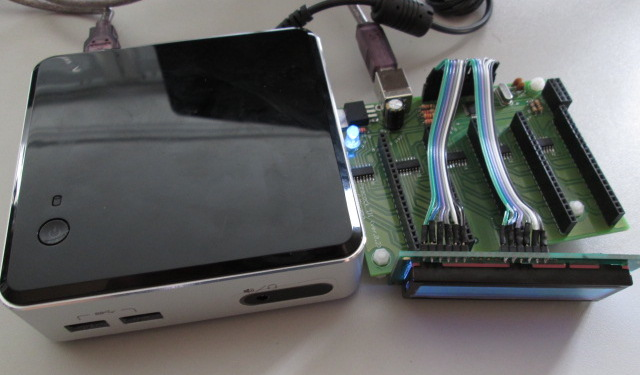
\includegraphics[width=1\columnwidth]{interface_main}
       \caption{interface board and main unit}
       \label{fig:interface_main}
\end{figure}

\section{Interface Board} % (fold)

The interface board is comprised of a Atmel AVR microcontroller, ATMega 32U2 and five external 12 bit ADCs, MCP3208, a LCD, 5 buttons and a LED. The main functionalities of the interface board are as follows:

\begin{enumerate}
       \item stabilization of the sensor power supply, employing onboard capacitors.
       \item data collection from the sensors and buttons, employing 5 external ADCs
       \item status indication of the peacock, using a LCD
       \item production of data packet 
       \item transfer of the data packets to the main computer via a USB cable, employing LUFA framework
\end{enumerate}

\begin{figure}[htbp]
       \centering
              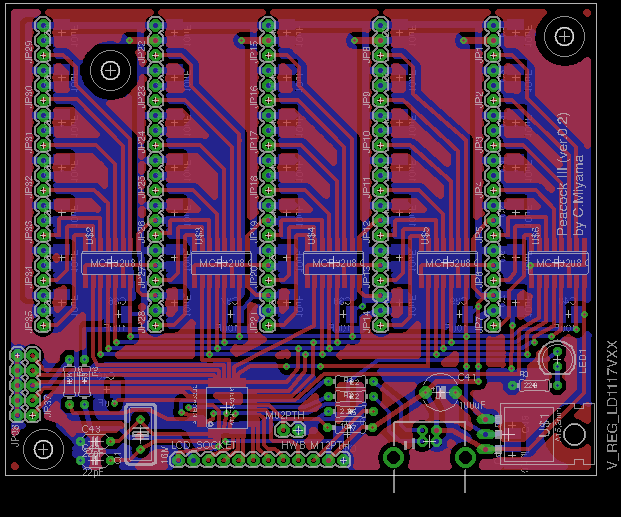
\includegraphics[width=1\columnwidth]{board}
       \caption{The PCB of Peacock III}
       \label{fig:board}
\end{figure}


\begin{figure}[htbp]
       \centering
              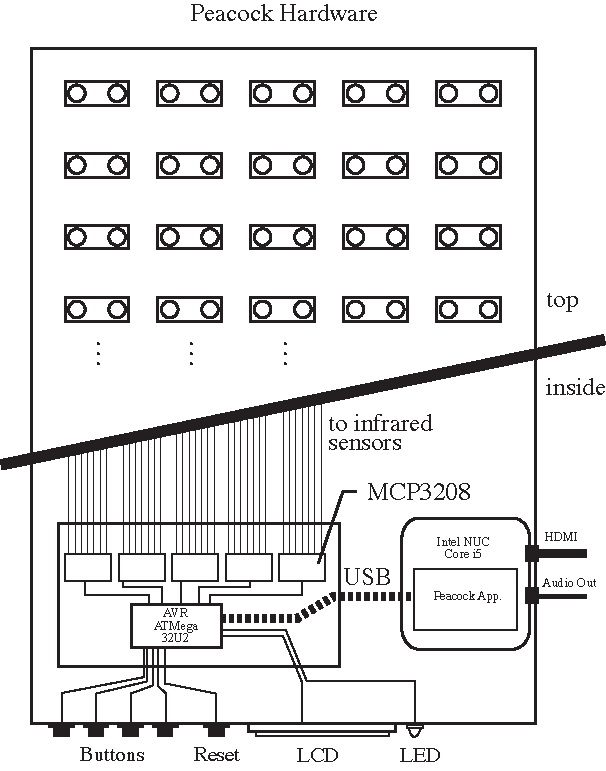
\includegraphics[width=1\columnwidth]{Peacock_hardware}
       \caption{The Peacock III Hardware}
       \label{fig:peacock}
\end{figure}


\subsubsection{Hardware signal stabilization} % (fold)

The signal from infrared sensors employed by Peacock include significant amount of noise. In Peacock I and II, the stabilisation of the signal took place in the software by applying digital low pass filters to all incoming signals, though the hardware level low pass filter is more preferable. On the PCB board of Peacock III, 35 SMD capcitors were employed for the  hardware-level stabilization of each incoming sigal.

\subsubsection{data collection} % (fold)

In order to collect data from all 35 infrared sensors, five 12 bit A/D converters are employed on the board and communicates with ATMega 32U2, using SPI(Serial Periferal Interface) protocol.

\subsubsection{Status indication/manipulation} % (fold)

A 2x16 LCD is attached on the side panel of the enclosure and it displays current status of the system. Users are able to change the setting of the system, and control the program for the sound generation, using this LCD and the buttons, placed next to the LCD.

\subsubsection{Production of safe data packet} % (fold)

A data packet always start with a start delimiter(0xFF), followed by a data type specifier, main data, and ended with a check sum. 

\subsection{transfer of the data packets} % (fold)

In Peacock I, a FTDI chip bridges the UART messages from the AVR microcontroller to the host computer.
However, by employing AVR ATMega 32U2, a microcontroller with a hardware USB controller, the newer version of Peacock is capable of sending data directly from the microcontroller to the host computer. For the development of the USB firmware, the LUFA (Lightweight USB Framework for AVRs)\cite{camera:lufa} was employed. The host computer recognize the Peacock PCB as a virtual serial device.

\section{Main Unit} % (fold)
A dedicated Intel NUC computer, ultra Compact Form factor computer with intel Corei5 processor placed next to the PCB board in the enclosure, runs Arch linux and automatically launch the PeacockApp, an OpenFrameworks\cite{openframeworks}-based application written in C++. This application receives the data from the microcontroller and send it to the following three modules. The gesture recognizer module analyze the incoming data and detects specific hand gesture, The synthesizer module is for sound production, and the visualizer module visualizes the incoming data.

\begin{enumerate}
       \item Gesture Recognizer(PckRecognizer)
       \item Synthesizer(PckSynthesizer)
       \item Visualizer(PckVisualizer)
\end{enumerate}

The Gesture Recognizer analyzes the incoming data, analyzes it with numerous different techniques and send a notification to the other two modules when it detect a new hand gesture\ref{fig:modules}.


\begin{figure}[htbp]
       \centering
              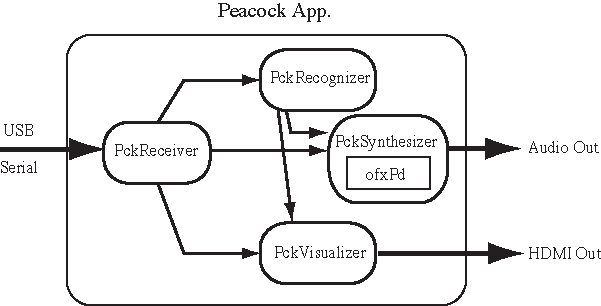
\includegraphics[width=1\columnwidth]{Peacock_app}
       \caption{The Peacock III App}
       \label{fig:modules}
\end{figure}

In order to minimize the latency and maximize the efficiency of the data processing, These three modules runs onthree separate threads in the application. If the Gesture Recognizer module detects a certain hand gesture, a notification will be sent immediately to the other two modules.


\subsection{Gesture Recognizer: PckRecognizer}

\subsubsection{Lower Level Analysis}

\begin{enumerate}
       \item Centroid X,Y
       \item Hand position
\end{enumerate}


\subsubsection{Higher Level Analysis}

\begin{enumerate}
       \item Centroid X,Y
       \item Hand position
\end{enumerate}

\subsection{Sound Generator: PckSynthesizer}

The sound generator modulede is currently programmed with Pd (Pure Data). ofxPd, an addon of oF(OpenFrameworks), enables the Peacock app to run Pd patches within the Peacock App. The Pd patches receives all data from the sensors, the result of analysis by the Gesture Recognizer, and the commands from buttons on the side panel and utilize it for the sound production.

\begin{figure}[htbp]
       \centering
              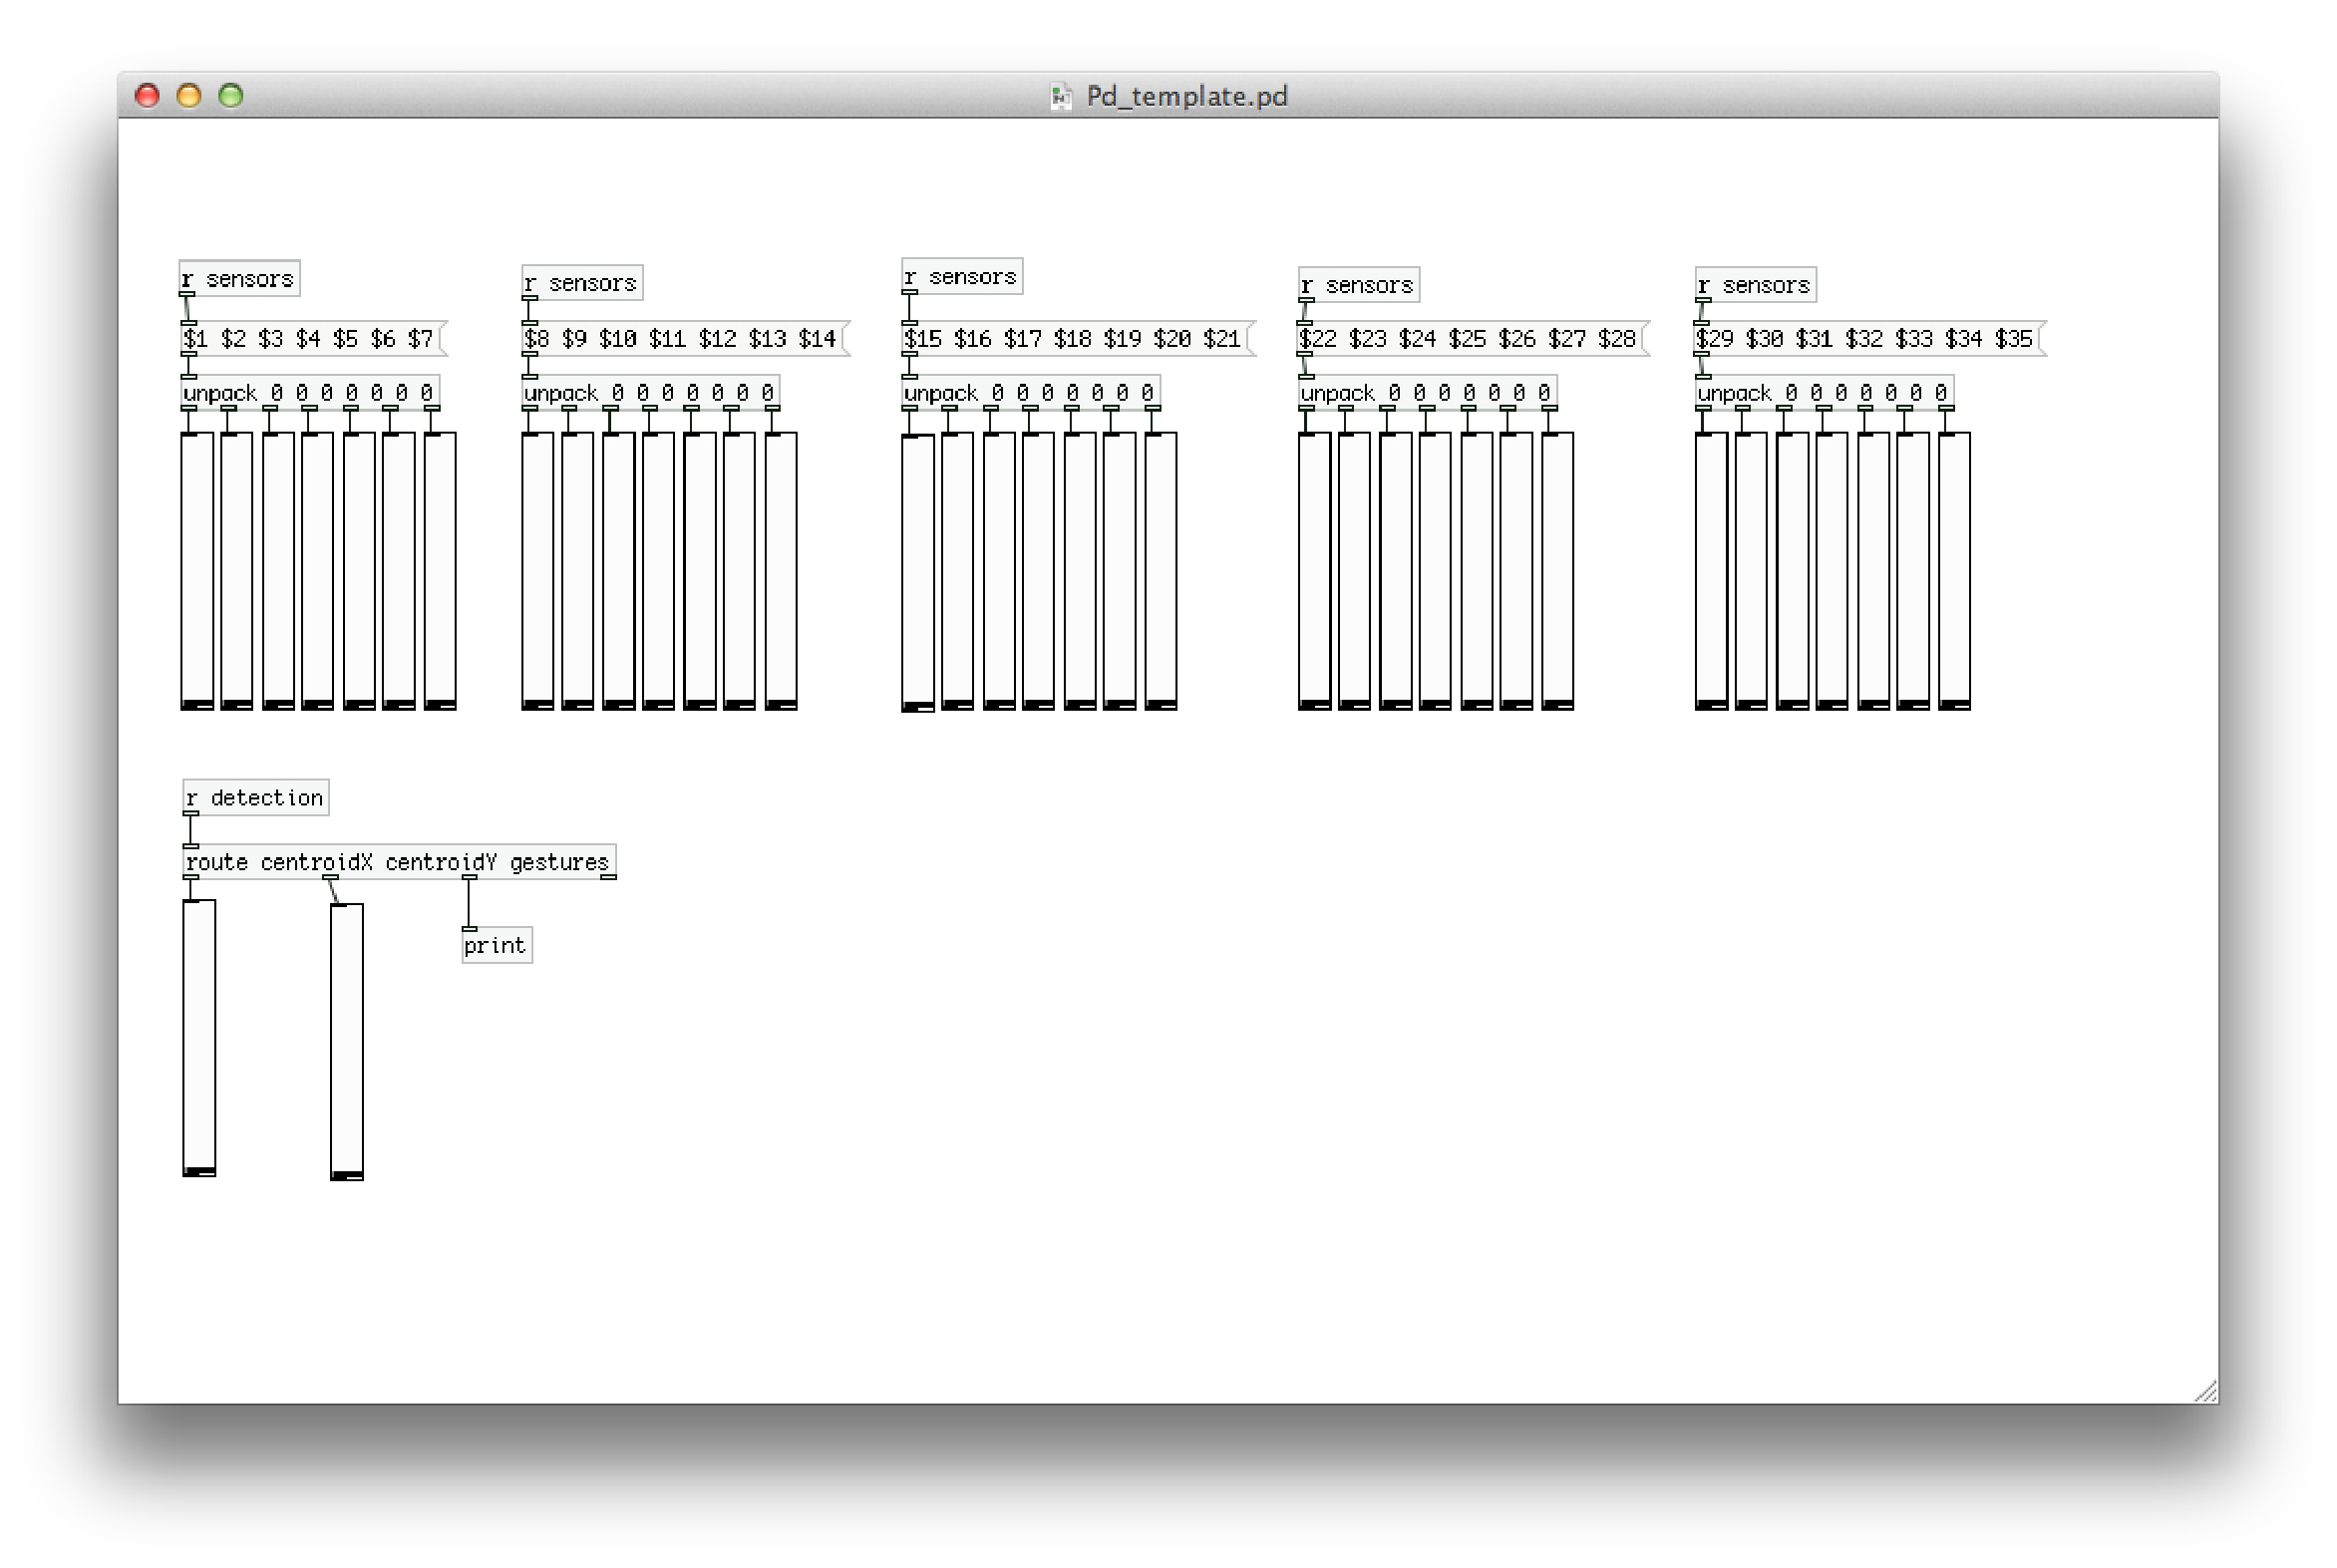
\includegraphics[width=1\columnwidth]{pd_patch}
       \caption{a template Pd Patch}
       \label{fig:modules}
\end{figure}
 
\subsection{Visualizer: PckVisualizer}

Unlike piano, cello, or other acoustic instruments, the player of Peacock controls musical parameters by simply moving hand above the device; There is no physical feedback from the instrument. In order to improve accurate parameter control, pricise positioning and movements of the hands is necessary. For this end, a visualizer provides the performer with optical feedback.  The visualizer indicates the values of from 35 infrared sensors  the assumed position of hands, chronological trail of hand movement, and recognized gestures, in  3D model programmed with OpenGL. The renderered 3D images can be displayed by attaching an optional HDMI-compatible monitor to the device.
The visualizer can be deactivated by the user by the buttons on the side of the enclosure.

\begin{figure}[htbp]
       \centering
              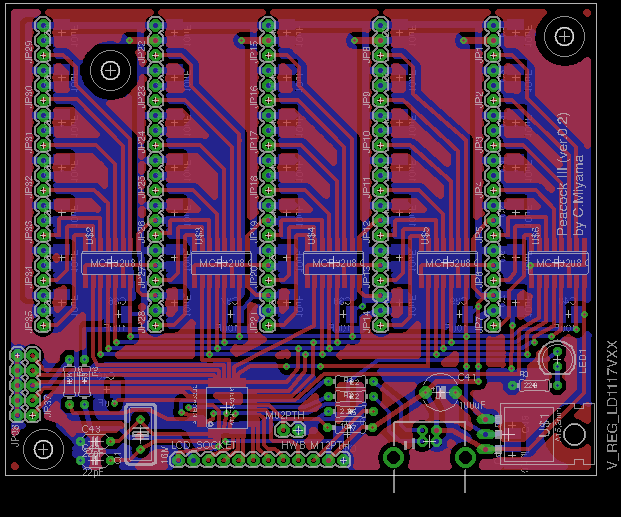
\includegraphics[width=1\columnwidth]{board}
       \caption{Visualizer}
       \label{fig:modules}
\end{figure}

\subsection{bandwidth}
The system is capable of capture the values from all sensors more than 1000 time per second.



\section{future works}

Further improvement of firmware and in the gesture recognition module is scheduled.
The source code of the PeacockApp and Peacock Firmware is hosted on github.com under GPL v3 lincense.


\section{acknowledgement}
This project is funded by fellowship program of the Academy of Media Arts Cologne. The author would like to express my sincere appreciation to Prof. Anthony Moore and Mr. Dirk Specht for their valuable support.

\bibliographystyle{abbrv}
\bibliography{KHM-references.bib}

\end{document}
